\documentclass[11pt]{article}
\usepackage{graphicx}
\usepackage[margin=1in]{geometry} %reducir márgenes
\usepackage{cite} %opciones entre {}
\pagestyle{empty} %quitar números de página
\usepackage{enumerate}

\setlength{\parskip}{8mm}

\parindent 0ex 
\renewcommand{\baselinestretch}{1.2} 

\begin{document}

\section*{\textbf{Anexo: Instalación glpk}}

Para realizar la instalación de la biblioteca glpk que vamos a usar para realizar las operaciones matematicas nos dirigimos a su página oficial : "https://www.gnu.org/software/glpk/" donde encontraremos la documentación y descargaremos su ultima versión (Figura \ref{fig:version}).

\begin{figure}[h!] 
\centering
    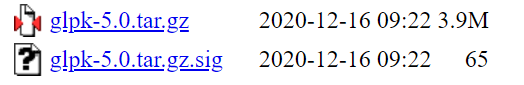
\includegraphics[width=0.4\textwidth]{img/version.PNG}
\caption{Versión GLPK}
\label{fig:version}
\end{figure}

Para realizar la instalación es necesario contar con un subsistema Linux, es necesario de cara a ejecutar algunos comandos. En nuestro caso hemos usado Debian que se puede descargar gratis en la Microsoft Store.

\section*{Descomprimir el archivo de distribución}

Una vez contamos con el entorno para ejecutar los comandos Abriremos el archivo INSTALL.txt donde se encuentran los pasos que hemos realizado.

\begin{enumerate}[1.]
\item Mover el archivo de distribución de glpk a la carpeta de trabajo
\item Descomprimir el archivo con el comando gzip -d glpk-X.Y.tar.gz (Que se renombrara a 'glpk-X.Y.tar').
\item extraer el archivo con el comando
\end{enumerate}

\begin{center}tar -x < glpk-X.Y.tar \end{center}

\section*{Configuración del paquete}

A continuación entraremos en la terminal de linux y accedremos al directorio donde se encuentre el archivo que acabos de extraer al ser un entorno en Linux debemos usar los comandos correspondientes para navegar por la terminal "cd" y "dir".

Una vez nos encontremos en la ruta de carpeta llamada glpk-5.0 ejecutaremos el script configure con el comando "./configure" (Figura \ref{fig:configure}).

\begin{figure}[h!] 
\centering
    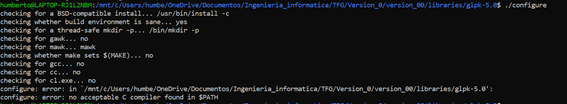
\includegraphics[width=1\textwidth]{img/configure.png}
\caption{Comando configure}
\label{fig:configure}
\end{figure}

En nuestro caso termino con error al no encontrar un compilador de C.

Intentamos ejecutar el comando "sudo apt-get install build-essential", pero retorno un error al no encontrar el paquete build-essential.

La solución fue añadir la línea "deb http://ftp.debian.org/debian stable main contrib non-free" en el archivo sources.list (Figura \ref{fig:sourceslist}). y ejecutar el comando "apt-get update.


\begin{figure}[h!] 
\centering
    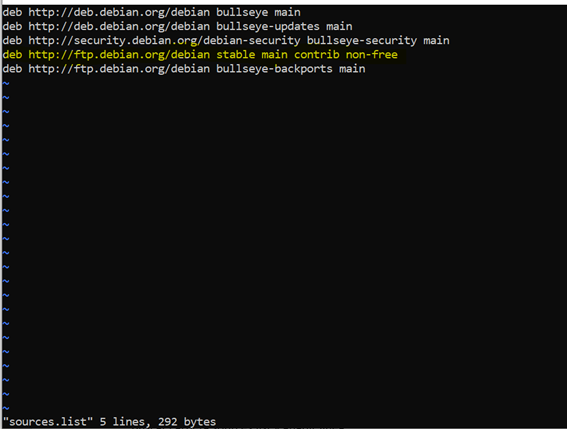
\includegraphics[width=1\textwidth]{img/sourceslist.png}
\caption{Archivo Sources List}
\label{fig:sourceslist}
\end{figure}

Al ejecutar de nuevo "sudo apt-get install build-essential" la configuración se realiza con éxito. 

Esta ejecución deberia tardar unos segundos y nos generara los siguientes archivos:

\begin{itemize}
    \item Makefile
    \item config.h: contiene datos dependientes de la plataforma
    \item config.status: script de shell que podemos ejecutar para recrear la confugración actual
    \item config.cache: guarda los resultados de los tests, accelerando el proceso de reconfiguración
    \item config.log: contiene salida del compilador
\end{itemize}

   

\section*{Compilación del paquete}

Unicamente tenemos el ejecutar el comando "make" que leera el archivo Makefile generado por el scriipt configure en el paso anterior y realizara los pasos necesarios.

Este comando permite algunas configuraciones como anular variables CFLAGS y LDFLAGS, o cambiar la ruta del directorio que contiene el código fuente, pero que en este caso no hemos necesitado utilizar.

\section*{Checkeo del paquete}

Podemos ejecutar algunos tests incluidos en el paquete, para verificar la correcta configuración y compilación con el comando:

\begin{center}make check \end{center}


\section*{Instalación del paquete}

El último paso de la instalación es el comando "make install" que por defecto instala los archivo del paquete en 'usr/local/bin', 'usr/local/lib' pudiendo cambiar esto path en caso de ser requerido

Despues de la instalación podemos eliminar los archivo ('Makefile','config.status',etc.) generados por el script configure, escribiendo el comando "make distclean".

Por último comentar que para desinstalar el paquete GLPK, podemos ejecutar el comando "make uninstall".

% comprobación instalación


\bibliographystyle{plain}
\bibliography{library}


\end{document}
